\section{A Lagrangian representative with controlled topology}
\label{top:section}

The obstruction calculation will use two properties of a Lagrangian
representative: ambient forms must detect its cohomology in degrees two
and six, and its Maslov grading must be defined modulo four.  We construct
these properties together.  All homology and cohomology in this section
have rational coefficients unless another coefficient ring is displayed.
The symplectic torus $T$, the class $\alpha$, and the space $\Omega$ are
those of Section~\ref{hodge:section}.

\begin{proposition}[The auxiliary brane]
\label{top:brane}
There are a positive integer $\nu$ and a closed connected oriented spin
Lagrangian embedding $i_L:L\hookrightarrow T$ such that
\begin{equation}\label{top:brane-class}
 (i_L)_*[L]=\nu\alpha.
\end{equation}
The embedding has a grading in the fourfold Maslov cover determined by
the standard complex volume form on $T$.  Moreover,
\begin{equation}\label{top:brane-cohomology}
 i_L^*:H^2(T)\longrightarrow H^2(L)
 \text{ is surjective},\qquad \ker i_L^*=\Omega,
\end{equation}
and
\begin{equation}\label{top:brane-injections}
 (i_L)_*:H_j(L)\longrightarrow H_j(T)
 \text{ is injective for }j=2,6.
\end{equation}
In particular, every form in $\Omega_{\C}$ restricts to an exact complex
two-form on $L$.
\end{proposition}

We first realize $\alpha$ by a stably framed manifold with the desired
cohomology, then use a local exact domain to control the signs of a
Lagrangian immersion.  The final surgeries preserve precisely the
homology groups in \eqref{top:brane-injections}.

\subsection{A nilmanifold and a framed representative}

Choose an integral basis $\eta_1,\ldots,\eta_{16}$ of a full lattice in
$\Omega$.  Let $b:H_{\R}\times H_{\R}\to\R^{16}$ be bilinear,
integral on the coordinate lattice, with
\[
 b(x,y)-b(y,x)=(\eta_1(x,y),\ldots,\eta_{16}(x,y)).
\]
For example, take the upper triangular part of each integral alternating
matrix.  The multiplication
\[
 (x,z)(y,w)=(x+y,z+w+b(x,y))
\]
makes $H_{\R}\oplus\R^{16}$ a simply connected two-step nilpotent
Lie group $N$.  Its integral points form a cocompact subgroup $\Gamma$.
Projection onto the first coordinate descends to
\[
 \pi:\mathcal N=\Gamma\backslash N\longrightarrow T.
\]
The universal cover of $\mathcal N$ is contractible; thus
$\mathcal N$ is a classifying space for $\Gamma$, and
$\Gamma\to\pi_1(T)$ is surjective.

\begin{lemma}\label{top:nilmanifold}
Pullback induces an isomorphism
\[
 H^2(\mathcal N)\cong \bigwedge^2 H^*/\Omega.
\]
There is a class $\widetilde\alpha\in H_8(\mathcal N)$ with
$\pi_*\widetilde\alpha=\alpha$.
\end{lemma}

\begin{proof}
Nomizu's Theorem~\cite[Theorem~1]{nomizu} computes real cohomology by
invariant forms.  The invariant complex is generated in degree one by
$H^*_{\R}$ and $z_1^*,\ldots,z_{16}^*$, with
$dH^*_{\R}=0$ and $dz_i^*=\eta_i$, after changing signs if necessary.
On $H^*_{\R}\otimes\langle z_i^*\rangle$, the differential is the
wedge map in Lemma~\ref{hodge:linear-algebra}, hence is injective.
It is also injective on $\bigwedge^2\langle z_i^*\rangle$: in
\[
 d(z_i^*\wedge z_j^*)=\eta_i\wedge z_j^*-\eta_j\wedge z_i^*,
\]
the independence of the $\eta_i$ detects every coefficient.  These two
images have different central degrees and cannot cancel.  The closed
two-forms are therefore the horizontal ones, modulo the boundaries
$\Omega_{\R}$.

Dually, the horizontal Lie chain $\alpha\in\bigwedge^8H$ has boundary
\[
 \partial\alpha=\pm\sum_i z_i\wedge\iota_{\eta_i}\alpha=0
\]
by Lemma~\ref{hodge:linear-algebra}.  Its image under projection is
$\alpha$.  Naturality of the invariant complex proves the lifting
statement over $\R$.  Both the cohomology pullback and the homology
pushforward are rational linear maps.  Their asserted kernel and image
statements consequently descend from $\R$ to $\Q$.
\end{proof}

\begin{lemma}\label{top:framed-source}
There are a closed connected stably framed eight-manifold $L_0$, a map
$f_0:L_0\to T$, and a positive integer $\nu$ such that
\[
 f_{0*}[L_0]=\nu\alpha,\qquad
 \chi(L_0)>(\nu\alpha)\cdot(\nu\alpha).
\]
The map is surjective on fundamental groups, has an additional free
circle generator mapping trivially to $T$, and satisfies
\eqref{top:brane-cohomology} and \eqref{top:brane-injections} with
$f_0$ in place of $i_L$.
\end{lemma}

\begin{proof}
Rational framed bordism maps isomorphically to rational homology: the
Pontryagin--Thom identification and the framed-bordism spectral sequence
give this because the positive stable stems of the sphere are torsion
\cite[proof of Proposition~3.1]{framed-rational}.  Clearing denominators
therefore represents $\nu\widetilde\alpha$, for some positive integer
$\nu$, by a closed stably framed eight-manifold mapped to $\mathcal N$.

Perform the following surgeries over $\mathcal N$.  First connect the
components by framed one-handles and add loops mapping to a finite
generating set of $\Gamma$, making the fundamental-group map
surjective.  Its kernel is normally finitely generated, since both
groups are finitely presented.  Represent normal generators by disjoint
embedded circles and perform framed surgery on them, using their null
homotopies in $\mathcal N$.  The normal rank is seven; twisting a
normal framing by $\pi_1\mathrm{SO}(7)$ makes it compatible with the
given stable framing.  The resulting fundamental group is $\Gamma$.

Next, $\pi_2$ of the source is finitely generated as a
$\Z\Gamma$-module.  Indeed, Hurewicz identifies it with the second
homology of the universal cover.  The cellular chain modules of that
cover are finite free over $\Z\Gamma$, and this ring is Noetherian
because $\Gamma$ is finitely generated nilpotent, hence polycyclic
\cite{hall}.  Represent module generators by disjoint embedded
two-spheres, possible by general position in dimension eight.  Their
normal bundles have rank six and are stably trivial, hence trivial;
the stable framing extends over surgery since $\pi_2\mathrm{SO}=0$.
The maps extend because $\pi_2(\mathcal N)=0$.  The reverse handles
have indices at least six, so these surgeries kill $\pi_2$ without
altering $\pi_1$.  All these modifications are bordisms over
$\mathcal N$ and preserve the pushed fundamental class.

The resulting source has two-connected universal cover.  Its
classifying map to $\mathcal N$ induces an isomorphism on $H^2$,
as follows, for example, from the low-degree homology sequence of the
universal-cover fibration.  Now take a framed connected sum with
$S^1\times S^7$ and with sufficiently many copies of
$S^4\times S^4$, mapping the added summands constantly.  These
products are stably parallelizable.  The first summand supplies the
extra null-image generator, while each of the latter summands raises
the Euler characteristic by two.  None changes $H^2$.  Call the
resulting map to $T$ $f_0:L_0\to T$.

Lemma~\ref{top:nilmanifold} now gives the surjectivity and kernel in
\eqref{top:brane-cohomology}.  Duality gives injectivity on $H_2$.
For $u\in H_6(L_0)$, Poincar\'e duality and that same surjectivity
write $u=f_0^*\eta\cap[L_0]$ for some $\eta\in H^2(T)$.  Then
\[
 f_{0*}u=\eta\cap(\nu\alpha)=\nu\iota_\eta\alpha.
\]
If this vanishes, Lemma~\ref{hodge:linear-algebra} puts $\eta$ in
$\Omega$, so $u=0$.  This proves the $H_6$ injection.
\end{proof}

\subsection{A graded immersion and its branch actions}

Since $\omega\in\Omega$, we have $f_0^*[\omega]=0$ over $\R$.
The stable real framing gives a stable complex trivialization of
$TL_0\otimes\C$ with trivial determinant phase on the oriented real
tangent.  Rank eight is in the unitary stable range over an
eight-dimensional manifold, so this trivialization can be
destabilized, preserving its stable homotopy class.  Its restriction
to $TL_0$ is a Lagrangian bundle monomorphism into the trivial
symplectic bundle $f_0^*TT$, of Maslov class zero.  The
Gromov--Lees immersion theorem, with its cohomological hypothesis
$f_0^*[\omega]=0$, realizes it by a Lagrangian immersion homotopic to
$f_0$ \cite[Theorem~2.3]{gromov-lees}.  Choose its integral grading
with the parity corresponding to the given orientation.

For such an immersion $f$, let $K_f$ be the kernel of
$\pi_1(L_0)\to\pi_1(T)$.  A loop representing $\gamma\in K_f$
has a filling in $T$, and its symplectic area defines
$\mathcal A_f(\gamma)\in\R$.  This is independent of the filling
because $\pi_2(T)=0$, and of the representative because $f$ is
Lagrangian.  Concatenation makes $\mathcal A_f$ additive on $K_f$;
transport and conjugation do not change it.

\begin{lemma}\label{top:zero-actions}
After Lagrangian perturbations of $f$ there is a self-transverse
immersion $f_1$ without triple points, still integrally graded and
homotopic to $f_0$, with the following property.  Its double points
can be written $f_1(a_j)=f_1(b_j)$, and there are pairwise disjoint
embedded arcs from $a_j$ to $b_j$ whose image loops are contractible
in $T$ and have area zero.
\end{lemma}

\begin{proof}
The action subgroup contains $1$.  To see this, lift based loops
mapping to lattice vectors $v,w$ with $\omega(v,w)=1$; this is
possible by fundamental-group surjectivity.  Their commutator lies
in $K_f$, and integration of $-p^t dq$ on the universal cover gives
its area as $\pm\omega(v,w)$: the translated opposite sides cancel
except for this lattice pairing.

The extra circle of Lemma~\ref{top:framed-source} admits an
independently adjustable action.  In an immersed cotangent
neighborhood of $f$, replacing the zero section by a small closed
one-form changes its action by that form's period, up to sign.
Choose this period so that the resulting action is irrational.
The action subgroup then contains $\Z+\rho\Z$ with
$\rho\notin\Q$, and is dense in $\R$.  Small exact perturbations
on source patches make the immersion self-transverse without triple
points; they do not change these loop periods.

For each double point choose a path $a_j\to b_j$.  By inserting a
loop at $a_j$, fundamental-group surjectivity first makes its image
contractible.  Inserting an element of $K_f$ then makes its filling
area arbitrarily small.  Choose mutually disjoint small source
patches at the $a_j$, avoiding the other double-point preimages.
An exact perturbation by $dF_j$, where $F_j$ is constant near $a_j$
and zero outside its patch, fixes the sheet near the double point
but changes this path action by $F_j(b_j)-F_j(a_j)$, up to the
fixed sign convention.  Thus it makes the action exactly zero.
This endpoint formula remains valid if a chosen path revisits the
patch.  For the fixed patches there is a uniform smallness bound
preserving all transverse double points and introducing no new
ones; choose the preceding residual areas within that bound.

Finally, relative homotopies of these paths preserve their actions.
General position in the eight-dimensional source makes them
embedded, pairwise disjoint, and disjoint from every other
double-point preimage.
\end{proof}

The algebraic number of double points of $f_1$ is
\begin{equation}\label{top:negative-index}
 I(f_1)=\frac{(\nu\alpha)\cdot(\nu\alpha)-\chi(L_0)}2<0.
\end{equation}
Indeed, the normal Euler number of an oriented Lagrangian
eight-manifold is $(-1)^{8\cdot7/2}\chi(L_0)=\chi(L_0)$, and
the self-intersection formula is the normal Euler number plus twice
the signed double-point count.

\subsection{An embedded exact domain containing the double points}

The next lemma makes the simply connected flexibility theorem
applicable inside a torus.  Its exactness and its embedding in $T$
are both part of the construction.

\begin{lemma}[The local exact domain]\label{top:exact-domain}
There is a compact contractible Weinstein domain
$(P,\lambda)\subset(T,\omega)$, with $d\lambda=\omega|_P$, such
that $W=f_1^{-1}(P)$ is a disk containing all double-point
preimages.  The Liouville vector field is tangent to its immersed
sheets, $f_1^*\lambda|_W=0$, and the immersion is cylindrical in
a collar of $\partial W$.  At one interior point of $W$ its image
is a single linear Lagrangian sheet in a radial Darboux ball.
\end{lemma}

\begin{proof}
Extend the arcs of Lemma~\ref{top:zero-actions} to a finite
embedded tree $\Theta\subset L_0$, using connector edges avoiding
all double-point preimages.  Set $G=f_1(\Theta)$.  The only
identifications on this tree are the paired endpoints $a_j,b_j$,
so $f_1^{-1}(G)=\Theta$.  Its graph cycles are freely generated
by the chosen arcs, with suitable connecting paths.  They are
contractible in $T$ and have filling area zero.  Subdivide an
ordinary edge to provide a vertex with just one preimage.

\paragraph{The zero- and one-handles.}
At every vertex take a small Darboux ball with radial Liouville
field.  A single sheet, or the two transverse sheets at a double
point, can be made linear simultaneously.  For the latter claim,
first make one sheet horizontal; the other is a gradient graph
over the vertical plane, and a symplectic shear straightens it
while fixing the first.  By homotoping the tree near its vertices,
make its incident edges distinct radial rays.  Join these balls by
thin Weinstein one-handles along the remaining arcs, carrying
Lagrangian strips in the corresponding sheets.

We describe the attachment and its relative neighborhood data,
also for later use with two-handles.  For index $k=1,2$, use
symplectic coordinates $(u,v,z)$ with $u,v\in\R^k$ and
$z\in\R^{2(8-k)}$.  The vector field
\begin{equation}\label{top:handle-field}
 Z_k=(-u,2v,z/2)
\end{equation}
is Liouville.  A handle box has $|u|\leq1$,
$|(v,z)|\leq\epsilon$, with negative face near $|u|=1$ and
core $v=z=0$.  It has a quadratic Lyapunov function with one
critical point of index $k$.  For $k=1$, the set $v=0$ with $z$
in a fixed Lagrangian plane is an invariant Lagrangian strip.

The contact neighborhood identifications at the attaching locus
may be made strict for the specified contact forms.  Here is the
needed refinement of the neighborhood theorem.  Choose, on each
side, a hypersurface containing the isotropic locus and tangent
to the contact plane along it.  The Reeb field is transverse on
a sufficiently small neighborhood; its flow writes the contact
form as $da+\beta$ on that neighborhood, with $d\beta$
symplectic on the slice.  Match the slices by the symplectic
isotropic neighborhood theorem using the prescribed tangent and
symplectic normal data.  The two slice primitives differ by a
closed form whose restriction to the attaching locus is zero.
Since the neighborhood retracts onto that locus, this difference
is $dg$, with $g=0$ there.  Shifting the Reeb coordinate by $g$,
with the appropriate sign, makes the identification strict.
This argument also applies to an entire Legendrian patch.
Extension along the Liouville flows gives a symplectic collar
identification preserving the primitive.

For the one-handles, choose the Legendrian patch identifications
using a transverse strip framing along each source arc.  Either
orientation of such a patch can be chosen.  Extend the prescribed
end germs over the strip by tubular coordinates.  The relative
Lagrangian neighborhood theorem extends this strip map
symplectically, keeping the collar germs: after the tangent map is
specified, the remaining linear lift choices are contractible,
and the tubular construction and Moser argument are relative to
the collars.  On shrinking the handles, they are embedded,
mutually disjoint away from their prescribed attachments, and
meet no other sheets.  This follows from compactness and
$f_1^{-1}(G)=\Theta$.  Transport the model primitives through
these embeddings and glue them by the strict collars.

Rounding the positive corners transversely to the Liouville field
gives an embedded Weinstein zero- and one-handlebody $P_1$ with
spine $G$.  Its preimage thickens the original tree $\Theta$,
hence is a disk.  The field is tangent to every sheet there;
equivalently, the primitive restricts to zero.  Its boundary is
therefore Legendrian and has the required positive cylindrical
collar.  The chosen single-sheet vertex retains a smaller radial
Darboux ball.

\paragraph{Exterior isotropic disks.}
The inclusions
\[
 \partial P_1\longrightarrow P_1,
 \qquad T\setminus\operatorname{int}P_1\longrightarrow T
\]
induce isomorphisms on fundamental groups.  For the first this is
the dual handle decomposition of a sixteen-dimensional zero-
and one-handlebody; for the second, attaching the removed
handlebody from its boundary involves only indices fifteen and
sixteen.  Choose loops giving a free basis of $\pi_1(P_1)$ in
$\partial P_1$.  The relative subcritical isotropic embedding
$h$-principle in contact manifolds
\cite[Theorem~12.4.1]{gromov-flexibility}
makes them disjoint isotropic circles, avoiding the Legendrian
boundary of the immersed disk.  The required formal tangent
lines can be deformed into the contact hyperplanes, and all the
avoidance conditions are in the general-position range.

Each circle bounds a smooth disk outside $P_1$: its class maps
trivially to $\pi_1(T)$, hence to the fundamental group of the
exterior.  Prescribe as its initial collar the outward
Liouville-flow cylinder, which is isotropic.  General position
relative to these collars gives embedded disks with mutually
disjoint interiors, avoiding the immersed eight-manifold; here
$2+2<16$ and $2+8<16$.

Each disk has symplectic area zero.  Indeed an annulus in $P_1$
joins its boundary to the corresponding graph cycle.  The
$\lambda$-integral on both boundary curves is zero: one is
isotropic in the contact boundary and the other lies in the
Lagrangian sheets where $f_1^*\lambda=0$.  The annulus therefore
has zero area.  The graph cycle has a zero-area filling by its
construction, and $\pi_2(T)=0$ makes the area independent of
the chosen filling.

We need isotropic disks, with the already prescribed collars.
The following formal check ensures that the subcritical
$h$-principle supplies them.  Take a prequantization circle bundle
of the integral symplectic form $\omega$, with its contact
connection.  The isotropic disk collars lift horizontally.  The
zero filling area makes their holonomy trivial and, in a
trivialization over each disk, gives winding number zero for the
boundary lift.  Thus these horizontal lifts extend to smooth
lifts of the disks.  This uses area zero, rather than merely an
integral area.

Trivialize the contact bundle over each lifted disk.  The space
of isotropic ordered two-frames retracts to $\mathrm U(8)/\mathrm
U(6)$, whose fundamental group is zero.  The prescribed
isotropic tangent frames on the collar consequently extend
over the disk.  The ordinary real two-frame space in rank
seventeen is two-connected, so the lifted disk derivative is
homotopic, relative to that collar, to this isotropic
monomorphism.  The relative, $C^0$-dense subcritical contact
embedding $h$-principle now realizes the formal data
\cite[Theorem~12.4.1]{gromov-flexibility}.  Fix a slightly narrower collar
throughout.  The approximations preserve avoidance by
$C^0$-smallness away from it.

Projection to $T$ is an isotropic immersion.  It may be chosen
embedded, with all the disks disjoint.  In fact contact
Hamiltonian perturbations supported near distinct lift points
give independently arbitrary projected variations, so projected
double points and intersections are removed by transversality
in dimension sixteen.  The same argument preserves avoidance
of $f_1(L_0)$, and the fixed narrower collars protect the
attachments.  We have therefore obtained actual disjoint
isotropic core disks in the exterior, relative to the required
germs.

\paragraph{The two-handles.}
Attach the model \eqref{top:handle-field} with $k=2$ along these
cores.  Its symplectic normal quotient along the attaching
circle is the contact conformal symplectic normal bundle,
with scale fixed by the contact form.  Choose its attaching
framing from a symplectic normal framing over the core disk,
and its parameterization from one extending over that disk.
Thus both the tangent and normal data of the prescribed collar
identification extend.  The relative isotropic neighborhood
theorem, followed by relative Moser, embeds a sufficiently thin
actual handle with that collar germ.  These handles miss the
immersion; their primitives glue by the strict identifications
above.  Rounding corners gives the desired domain $P$.

Topologically, $P$ is the graph $G$ with a two-cell attached
along each free generator, hence is contractible.  More
explicitly, after collapsing a maximal tree its attaching maps
are a free basis of a bouquet of circles, so this two-complex
is homotopy equivalent to a point.  The two-handles are
disjoint from the immersion, so its preimage remains the disk
already constructed in $P_1$.  The primitive, collar, and
radial single-sheet ball remain unchanged.
\end{proof}

\begin{figure}[tb]
\centering
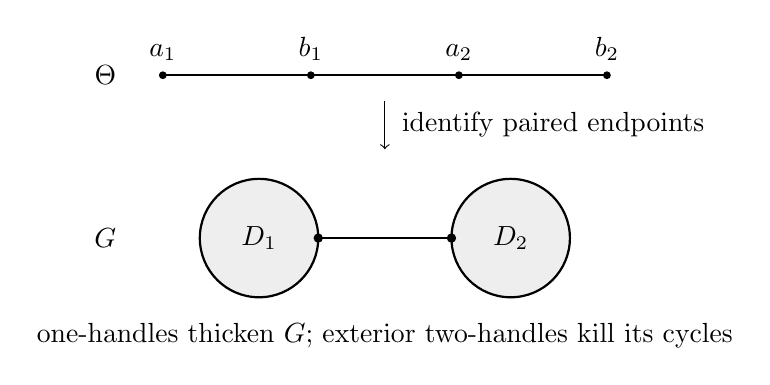
\begin{tikzpicture}[x=1cm,y=1cm,scale=.94]
 \draw[thick] (.4,2.2)--(6.4,2.2);
 \foreach \x/\s in {0.4/a_1,2.4/b_1,4.4/a_2,6.4/b_2}
   {\fill (\x,2.2) circle (1.5pt);\node[above] at (\x,2.27) {$\s$};}
 \node[left] at (-.1,2.2) {$\Theta$};
 \draw[->] (3.4,1.85)--(3.4,1.2);
 \node[right] at (3.5,1.53) {identify paired endpoints};
 \fill[gray!13] (1.7,0) circle (.8);
 \fill[gray!13] (5.1,0) circle (.8);
 \draw[thick] (1.7,0) circle (.8);
 \draw[thick] (5.1,0) circle (.8);
 \draw[thick] (2.5,0)--(4.3,0);
 \fill (2.5,0) circle (1.8pt);
 \fill (4.3,0) circle (1.8pt);
 \node at (1.7,0) {$D_1$};
 \node at (5.1,0) {$D_2$};
 \node[left] at (-.1,0) {$G$};
 \node[below,align=center] at (3.4,-1.02)
   {one-handles thicken $G$; exterior two-handles kill its cycles};
\end{tikzpicture}
\caption{The topology of the local domain, illustrated with two double
points.  The preimage tree thickens to an eight-disk.  The shaded disks
indicate the two-handle attachments only: their actual isotropic cores
attach to circles in $\partial P_1$ and lie off the immersed sheets.}
\label{top:domain-figure}
\end{figure}

\subsection{Removing positive double points and extending the grading}

\begin{lemma}\label{top:negative-doubles}
The immersion can be replaced on the disk $W$ by an oriented spin
Lagrangian immersion with only negative transverse double points.
It retains the boundary collar, its fundamental class, its integral
Maslov grading, and the homology-map properties in
Lemma~\ref{top:framed-source}.
\end{lemma}

\begin{proof}
Complete $P$ by its positive cylindrical end and extend the
immersed disk by its cylinder.  Remove the center of the
single-sheet radial ball supplied by Lemma~\ref{top:exact-domain}.
The punctured ball is a negative Liouville end.  The source
becomes an annulus $S^7\times\R$, with standard real-plane
Legendrian link $\phi_0\subset S^{15}$ at the negative end.
The punctured completion is simply connected, since removing
a point from a sixteen-manifold does not affect $\pi_1$.

We use the stabilization traces of
\cite[Lemma~3.2 and proof of Lemma~3.4]{eems}.  In source
dimension $2k$, a trace going outward from a Legendrian link
$\phi$ to its loose stabilization $\phi_1$ has one double
point of sign $(-1)^{k-1}$; the reverse trace has sign
$(-1)^k$.  For $k=4$ the signs are therefore
\begin{equation}\label{top:trace-signs}
 \phi\longrightarrow\phi_1:\ -1,
 \qquad \phi_1\longrightarrow\phi:\ +1.
\end{equation}
Put $m=-I(f_1)>0$.  Insert $m$ reverse traces in separated
radial collars near the puncture, ordered from the $m$-fold
stabilization $\phi_m$ at the innermost end to $\phi_0$
outward.  The negative link is now loose and the total signed
double count is $I(f_1)+m=0$.

Apply Eliashberg--Murphy's exact cancellation theorem
\cite[Theorem~2.3]{em-caps}.  Its hypotheses here are as
follows: the target is a simply connected Liouville manifold
with a negative end; the immersion is proper, self-transverse,
and has finitely many double points; its connected source has
dimension eight; the negative asymptote has one loose
component; and its signed double count is zero.  The
immersion is exact because $H^1(S^7\times\R;\R)=0$.
The additional width assumption of that theorem applies
only in source dimension three.  Its conclusion is a
compactly supported Hamiltonian regular homotopy to an
embedding.  Compact support preserves both cylindrical
tails, including the prescribed positive tail.

In the unchanged negative region, insert $m$ forward traces
from $\phi_0$ to $\phi_m$ and fill the center by the real
plane.  Equation~\eqref{top:trace-signs} shows that the filled
immersion has exactly $m$ double points, all negative.  Its
noncylindrical part is compact.  Apply a sufficiently long
negative Liouville flow in the filled positive completion to
bring this compact part inside $P$.  Backward flow exists
for all time; points inside $P$ cannot leave it backward,
and on the positive end it translates the cylindrical
coordinate.  The flow rescales the symplectic form, so
preserves Lagrangianity.  The positive cylinder remains the
same cylinder as a subset and crosses $\partial P$ in the
original collar.  Trim there and glue to the unmodified
immersion outside $W$.

The replaced source piece is a disk with collars.  A boundary
parameterization extends to a homeomorphism of disks, so the
old and new maps can be compared continuously relative to
the common complement.  As $T$ is aspherical, this disk
replacement preserves the homotopy class and the fundamental
class.  It also preserves the degree-two and degree-six
homology maps through the common complement.  Orient the
replacement compatibly.  Spin extends because the boundary
$S^7$ has a unique spin structure.  Finally every first
homology class is represented off the replaced disk; the
Maslov class therefore remains zero.  Choose the integral
grading with the original orientation parity.
\end{proof}

\begin{proof}[Proof of Proposition~\ref{top:brane}]
Apply local Lagrangian surgery at the negative double points
of Lemma~\ref{top:negative-doubles}.  We spell out the
grading choice, since it is the reason for using period four.
In symplectic coordinates the two sheets are
$\R^8$ and $i\R^8$.  The handle is
\[
 (s,x)\longmapsto\gamma(s)x,\qquad x\in S^7,
\]
where $\gamma$ rounds a corner from the positive real ray
to the positive imaginary ray through the first quadrant,
or to the negative imaginary ray through the fourth
quadrant.  The first ray is traversed inward and the second
outward.  With the usual monotone corner shapes these are
embedded Lagrangian handles: tangent vectors in the sphere
directions pair trivially, and their symplectic pairing
with $\gamma' x$ vanishes because $x\perp T_xS^7$.

These handles glue orientably exactly at a negative double
point.  For the coordinate orientations the two planes have
positive intersection sign in dimension eight, whereas
the handle gives opposite relative orientation marks at
its two ends.  Thus the negative intersection condition is
precisely the required orientation agreement.

Identify the ambient Maslov cover over each surgery ball
with the standard one.  For the phase lift $\arg\det/\pi$, a handle tangent frame
has determinant proportional to $\gamma'\gamma^7$.
Its total phase changes along the two corners are
\begin{equation}\label{top:surgery-phases}
 +3\quad\hbox{and}\quad-3,
\end{equation}
respectively; see also \cite[Lemma~2.4]{ekholm-smith}.
For example, along the first corner the initial argument
is $\pi$ and the final argument is $4\pi$.
The integral lifts of the two original sheet phases differ
by an odd integer, because their orientation marks are
opposite.  The two residues in \eqref{top:surgery-phases}
are the two odd residues modulo four.  Consequently one
of the two handles extends the grading modulo four at
each double point.  The choices are independent in
disjoint surgery balls.  The unique spin structures on
their boundary seven-spheres also give spin extensions.

Let $i_L:L\hookrightarrow T$ be the resulting embedded
Lagrangian.  Each oriented local surgery preserves its
pushed fundamental class.  Removing the pairs of
eight-disks and inserting $S^7\times[0,1]$ changes neither
$H_2$, $H_6$, nor $H^2$: the isomorphisms through the
common complement follow directly from the relative
homology sequence and Mayer--Vietoris.  They intertwine
the maps to $T$.  Thus all the properties of
Lemma~\ref{top:framed-source} asserted in the proposition
survive.  Finally \eqref{top:brane-cohomology}, extended
to $\C$, and de Rham's Theorem give exactness of the
restricted forms in $\Omega_{\C}$.
\end{proof}

\begin{corollary}[Ambient detection]\label{top:ambient-detection}
Let $r=2$ or $6$, and let $u$ be a closed complex $r$-form on $L$.
If
\[
 \int_L i_L^*\eta\wedge u=0
 \quad\text{for every closed complex $(8-r)$-form $\eta$ on $T$},
\]
then $u$ is exact.
\end{corollary}

\begin{proof}
The displayed pairings say that
$(i_L)_*([u]\cap[L])=0$ in $H_{8-r}(T;\C)$.
The relevant injection in \eqref{top:brane-injections}
and Poincar\'e duality give $[u]=0$.
\end{proof}
